\documentclass{article}
\usepackage[utf8]{inputenc}
\usepackage{amssymb,amsfonts}
\usepackage{amsmath}
\usepackage{tikz}
\usetikzlibrary{shapes,arrows,positioning}
\usetikzlibrary{er,positioning,bayesnet}

\begin{document}

     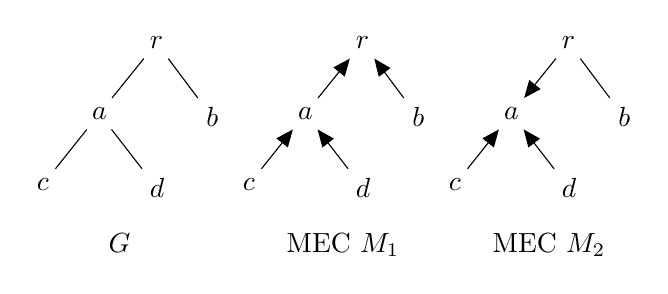
\begin{tikzpicture}
    \node[](r){$r$};
    \node[](a)[below left= 0.5 and 0.3 of r]{$a$};
    \node[](b)[below right = 0.5 and 0.3 of r]{$b$};
    \node[](c)[below left= 0.5 and 0.3 of a]{$c$};
    \node[](d)[below right = 0.5 and 0.3 of a]{$d$};
    \node[](G)[below left = 0.2 and 0.0 of d]{$G$};
    
    \draw[-](r)--(a);
    \draw[-](r)--(b);
    \draw[-](a)--(c);
    \draw[-](a)--(d);

    \node[](r1)[right = 2.2 of r]{$r$};
    \node[](a1)[below left= 0.5 and 0.3 of r1]{$a$};
    \node[](b1)[below right = 0.5 and 0.3 of r1]{$b$};
    \node[](c1)[below left= 0.5 and 0.3 of a1]{$c$};
    \node[](d1)[below right = 0.5 and 0.3 of a1]{$d$};
    \node[](G1)[below left = 0.2 and -0.8 of d1]{MEC $M_1$};
    
    \draw[<-](r1)--(a1);
    \draw[<-](r1)--(b1);
    \draw[<-](a1)--(c1);
    \draw[<-](a1)--(d1);

    \node[](r2)[right = 2.2 of r1]{$r$};
    \node[](a2)[below left= 0.5 and 0.3 of r2]{$a$};
    \node[](b2)[below right = 0.5 and 0.3 of r2]{$b$};
    \node[](c2)[below left= 0.5 and 0.3 of a2]{$c$};
    \node[](d2)[below right = 0.5 and 0.3 of a2]{$d$};
    \node[](G2)[below left = 0.2 and -0.8 of d2]{MEC $M_2$};
    
    \draw[->](r2)--(a2);
    \draw[-](r2)--(b2);
    \draw[<-](a2)--(c2);
    \draw[<-](a2)--(d2);
    \end{tikzpicture}

\end{document}